\def\DoNotLoadEpstopdf{}
\documentclass[tikz,border=14pt]{standalone}
\usepackage[T1]{fontenc}
\usetikzlibrary{arrows.meta,calc,positioning}

\definecolor{navy}{HTML}{182840}
\definecolor{blue}{HTML}{2757A4}
\definecolor{teal}{HTML}{10675E}
\definecolor{amber}{HTML}{8C5417}
\definecolor{line}{HTML}{526579}

\begin{document}
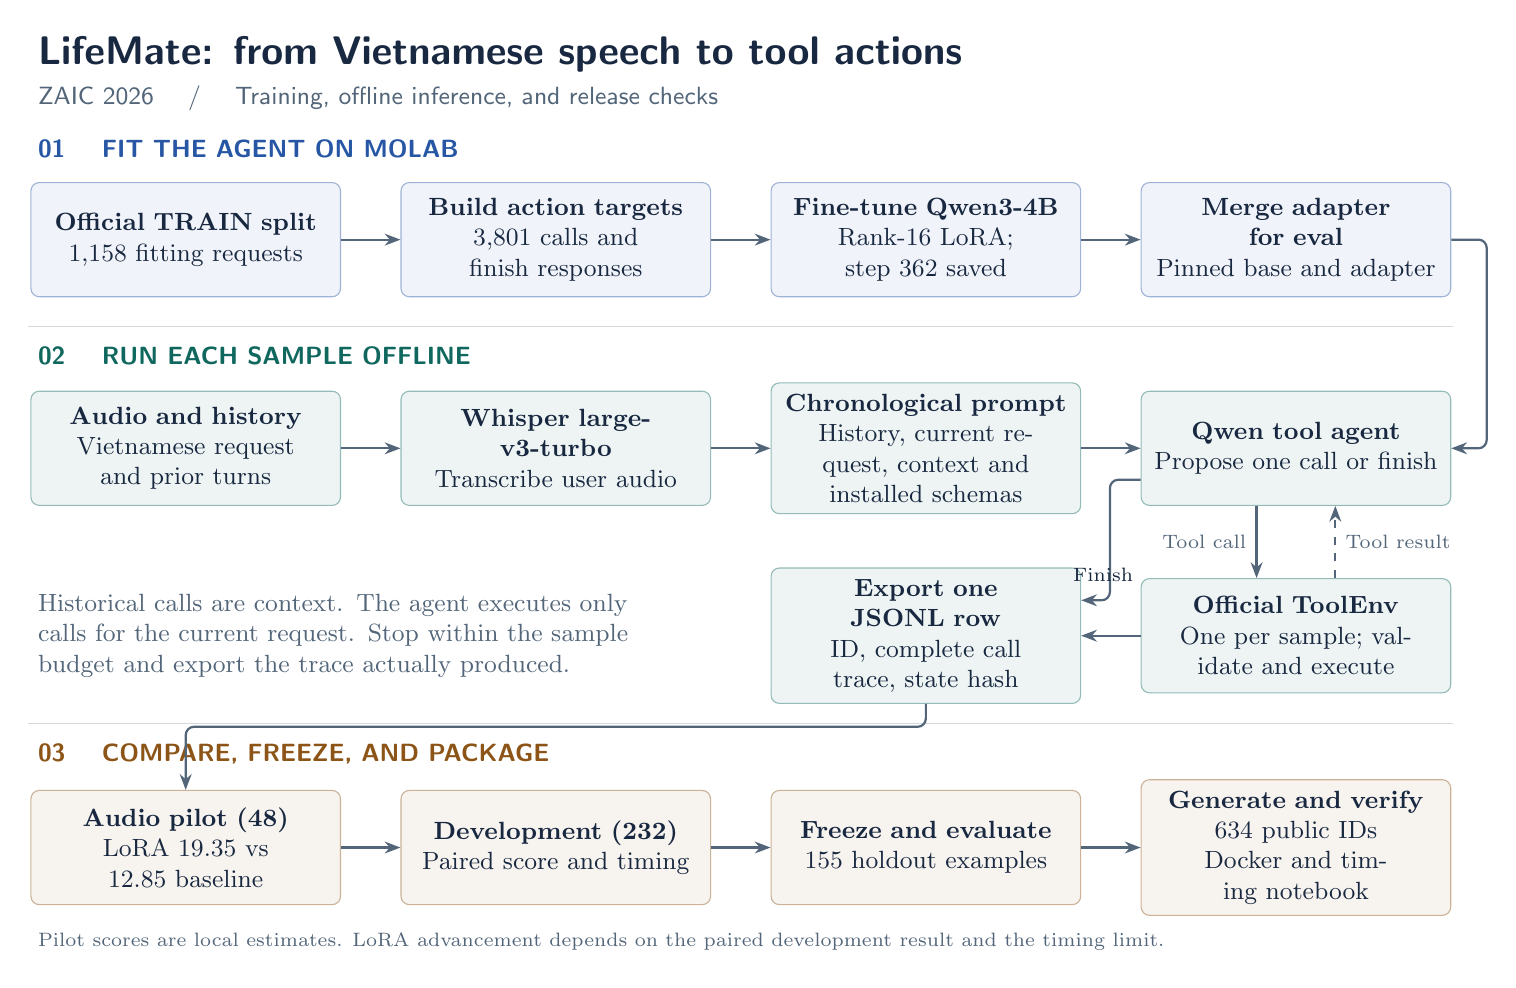
\begin{tikzpicture}[
  font=\sffamily, text=navy,
  stage/.style={anchor=west,font=\sffamily\bfseries\small},
  box/.style={draw=#1!45,fill=#1!7,rounded corners=3pt,align=center,
              text width=3.65cm,minimum height=1.45cm,inner sep=4pt,font=\small},
  flow/.style={-{Stealth[length=2mm]},line,thick,rounded corners=3pt},
  feedback/.style={flow,dashed},
  rule/.style={line!25},
]
\node[anchor=west,font=\sffamily\bfseries\Large] at (-2,1.35) {LifeMate: from Vietnamese speech to tool actions};
\node[anchor=west,font=\sffamily\small,text=line] at (-2,0.8) {ZAIC 2026 \quad / \quad Training, offline inference, and release checks};

\node[stage,text=blue] at (-2,0.15) {01 \quad FIT THE AGENT ON MOLAB};
\node[box=blue] (fit) at (0,-1) {\textbf{Official TRAIN split}\\1,158 fitting requests};
\node[box=blue] (targets) at (4.7,-1) {\textbf{Build action targets}\\3,801 calls and finish responses};
\node[box=blue] (lora) at (9.4,-1) {\textbf{Fine-tune Qwen3-4B}\\Rank-16 LoRA; step 362 saved};
\node[box=blue] (merge) at (14.1,-1) {\textbf{Merge adapter for eval}\\Pinned base and adapter};
\draw[flow] (fit) -- (targets);
\draw[flow] (targets) -- (lora);
\draw[flow] (lora) -- (merge);

\draw[rule] (-2,-2.1) -- (16.1,-2.1);
\node[stage,text=teal] at (-2,-2.48) {02 \quad RUN EACH SAMPLE OFFLINE};
\node[box=teal] (audio) at (0,-3.65) {\textbf{Audio and history}\\Vietnamese request and prior turns};
\node[box=teal] (asr) at (4.7,-3.65) {\textbf{Whisper large-v3-turbo}\\Transcribe user audio};
\node[box=teal] (context) at (9.4,-3.65) {\textbf{Chronological prompt}\\History, current request, context and installed schemas};
\node[box=teal] (agent) at (14.1,-3.65) {\textbf{Qwen tool agent}\\Propose one call or finish};
\node[box=teal] (env) at (14.1,-6.03) {\textbf{Official ToolEnv}\\One per sample; validate and execute};
\node[box=teal] (jsonl) at (9.4,-6.03) {\textbf{Export one JSONL row}\\ID, complete call trace, state hash};
\draw[flow] (audio) -- (asr);
\draw[flow] (asr) -- (context);
\draw[flow] (context) -- (agent);
\draw[flow] (merge.east) -- ++(0.45,0) |- (agent.east);
\draw[flow] ([xshift=-0.5cm]agent.south) -- node[left,font=\scriptsize] {Tool call} ([xshift=-0.5cm]env.north);
\draw[feedback] ([xshift=0.5cm]env.north) -- node[right,font=\scriptsize] {Tool result} ([xshift=0.5cm]agent.south);
\draw[flow] ([yshift=-0.4cm]agent.west) -- ++(-0.39,0) |- ([yshift=0.45cm]jsonl.east);
\node[font=\scriptsize,above] at (11.65,-5.47) {Finish};
\draw[flow] (env.west) -- (jsonl.east);
\node[align=left,font=\small,text=line,anchor=west,text width=8.2cm] at (-2,-6.03)
  {Historical calls are context. The agent executes only calls for the current request. Stop within the sample budget and export the trace actually produced.};

\draw[rule] (-2,-7.14) -- (16.1,-7.14);
\node[stage,text=amber] at (-2,-7.53) {03 \quad COMPARE, FREEZE, AND PACKAGE};
\node[box=amber] (pilot) at (0,-8.72) {\textbf{Audio pilot (48)}\\LoRA 19.35 vs 12.85 baseline};
\node[box=amber] (dev) at (4.7,-8.72) {\textbf{Development (232)}\\Paired score and timing};
\node[box=amber] (audit) at (9.4,-8.72) {\textbf{Freeze and evaluate}\\155 holdout examples};
\node[box=amber] (release) at (14.1,-8.72) {\textbf{Generate and verify}\\634 public IDs\\Docker and timing notebook};
\draw[flow] (jsonl.south) -- ++(0,-0.29) -| (pilot.north);
\draw[flow] (pilot) -- (dev);
\draw[flow] (dev) -- (audit);
\draw[flow] (audit) -- (release);
\node[anchor=west,font=\scriptsize,text=line] at (-2,-9.92)
  {Pilot scores are local estimates. LoRA advancement depends on the paired development result and the timing limit.};
\end{tikzpicture}
\end{document}
